\documentclass[conference]{IEEEtran}
\usepackage{graphicx}
\usepackage{hyperref}
\usepackage{cleveref}
\usepackage{url}
\usepackage{algorithm}
\usepackage{algpseudocode}
\usepackage{tikz}
\usepackage{booktabs}
\usetikzlibrary{arrows.meta, positioning, shapes.geometric, fit, backgrounds, calc}
\usepackage{listings}
\usepackage{xcolor}
\usepackage{multirow}
\usepackage{enumitem}
\usepackage{float}
\usepackage{amssymb}
\usepackage{ctex}
\algnewcommand{\Try}{\textbf{try}}
\algnewcommand{\Catch}{\textbf{catch}}
\algnewcommand{\EndTry}{\textbf{end try}}
\lstset{
    basicstyle=\ttfamily\small,
    breaklines=true,
    frame=single,
    numbers=left,
    numberstyle=\tiny\color{gray},
    keywordstyle=\color{blue},
    commentstyle=\color{green!60!black},
    stringstyle=\color{red},
    showstringspaces=false,
    tabsize=4,
    captionpos=b
}

\title{基于AI视觉理解的智能文档核验与自动盖章机器人系统}

\author{
\IEEEauthorblockN{Yaokai Yang }
\IEEEauthorblockA{\textit{School of Advanced Technology} \\
\textit{Xi'an Jiaotong-Liverpool University} \\
Suzhou, China \\
yaokai.yang23@student.xjtlu.edu.cn}
\and
\IEEEauthorblockN{Xiang Lin }
\IEEEauthorblockA{\textit{School of Advanced Technology} \\
\textit{Xi'an Jiaotong-Liverpool University} \\
Suzhou, China \\
xiang.lin23@student.xjtlu.edu.cn}
\and
\IEEEauthorblockN{Xinyang Zhang }
\IEEEauthorblockA{\textit{School of Advanced Technology} \\
\textit{Xi'an Jiaotong-Liverpool University} \\
Suzhou, China \\
xinyang.zhang23@student.xjtlu.edu.cn}
\and
\IEEEauthorblockN{Yunxuan Wu }
\IEEEauthorblockA{\textit{School of Advanced Technology} \\
\textit{Xi'an Jiaotong-Liverpool University} \\
Suzhou, China \\
yunxuan.wu23@student.xjtlu.edu.cn}
\and
\IEEEauthorblockN{Haoran Zheng }
\IEEEauthorblockA{\textit{School of Advanced Technology} \\
\textit{Xi'an Jiaotong-Liverpool University} \\
Suzhou, China \\
haoran.zheng23@student.xjtlu.edu.cn}
}

\date{2026年4月}

\begin{document}


\maketitle

\begin{abstract}
\textbf{项目摘要：}本项目提出并实现了一套\textbf{基于AI视觉理解的智能文档核验与自动盖章机器人系统}，面向行政办公、企事业单位及教育机构等场景中的文档审批自动化需求。系统采用\textbf{三层架构}设计——前端交互层、后台管理层与硬件执行层——将光学字符识别（OCR）、AI驱动的文档类型智能分类、基于RAG（检索增强生成）的知识辅助验证、多维规则引擎和舵机控制的物理盖章整合为统一的智能自动化流水线。系统完整实现了\textbf{输入 $\rightarrow$ 识别 $\rightarrow$ 推理 $\rightarrow$ 决策 $\rightarrow$ 执行 $\rightarrow$ 记录 $\rightarrow$ 分析}的全链路闭环。后台管理层提供可视化数据统计面板，涵盖审批通过率、文档类型分布、处理趋势分析及异常监测等核心运营指标。所有操作均生成包含盖章前后对比图的完整审计日志，确保全程可追溯。验证结果模糊的文件自动推入人工复审队列，实现\textbf{人机协同}审批。硬件总成本约240元，是一种低成本、高效率、可规模化复制的行政自动化解决方案。
\end{abstract}

%=============================================================================
\section{背景与动机}
%=============================================================================

\subsection{行业背景与问题描述}

在行政办公、企业审批、教育机构及政府服务窗口等场景中，文档处理——包括请假申请、费用报销、证明出具、合同签署等——长期依赖人工审核与物理盖章。据统计，行政人员在此类重复性文书工作上平均耗时超过30\%的工作时间。该流程面临以下核心挑战：

\begin{itemize}[leftmargin=*]
    \item \textbf{效率瓶颈：}工作人员必须逐份阅读文件、核对字段、物理盖章，每小时仅能处理10--15份文件，在业务高峰期易形成积压。
    \item \textbf{人为错误风险：}人工核验在疲劳状态下容易遗漏缺失字段、过期日期或身份信息不匹配等问题，错误率随工作量上升。
    \item \textbf{合规与审计缺失：}缺乏系统化的审计追踪机制，难以追溯审批时间线、责任归属和操作记录，存在问责空白。
    \item \textbf{印章安全漏洞：}物理印章经常无人看管，存在被未授权使用、复制或篡改的风险。
    \item \textbf{数据利用率低：}大量审批数据仅以纸质形式存档，未能转化为可分析、可优化的运营洞察。
\end{itemize}

\subsection{项目动机与技术契机}

随着AI视觉技术的成熟（如PaddleOCR等中文优化OCR引擎）、低成本微控制器（Arduino）的普及，以及检索增强生成（RAG）等技术在文档理解领域的应用探索，构建一个\textbf{智能化、低成本、可复制}的文档审批自动化系统已成为可能。本项目旨在：

\begin{enumerate}[leftmargin=*]
    \item 用\textbf{AI驱动的智能文档识别}替代人工文档审读，实现文档类型的自动分类与内容理解。
    \item 引入\textbf{RAG知识增强验证}机制，将OCR识别结果与机构政策、历史审批记录进行交叉检索，减少识别幻觉和误判。
    \item 通过舵机力度控制和防篡改锁定机构实现\textbf{物理盖章自动化}，确保盖章质量与安全性。
    \item 构建包含\textbf{可视化数据统计与运营分析}的后台管理平台，将审批数据转化为可量化的运营洞察。
    \item 提供\textbf{基于角色的Web界面}，实现操作员、复审员和管理员的权责分离与人机协同审批。
\end{enumerate}

\subsection{项目范围}

本项目为西交利物浦大学\textbf{MEC202 -- Specific General Project 9}课程项目，由陈邦翔博士指导。系统以高校行政场景为验证环境，针对四种典型文档类型（请假申请、费用报销、证明文件、通用文档）进行开发与测试。系统设计充分考虑\textbf{可扩展性}，支持通过模板管理机制灵活适配不同机构的文档类型与审批规则。

%=============================================================================
\section{系统方案与技术路线}
%=============================================================================

\subsection{系统总体架构}

系统采用\textbf{三层架构}设计，如\Cref{fig:architecture}所示。该架构将系统划分为三个协同工作的层次，实现从用户交互到物理执行的完整闭环：

\begin{figure}[H]
\centering
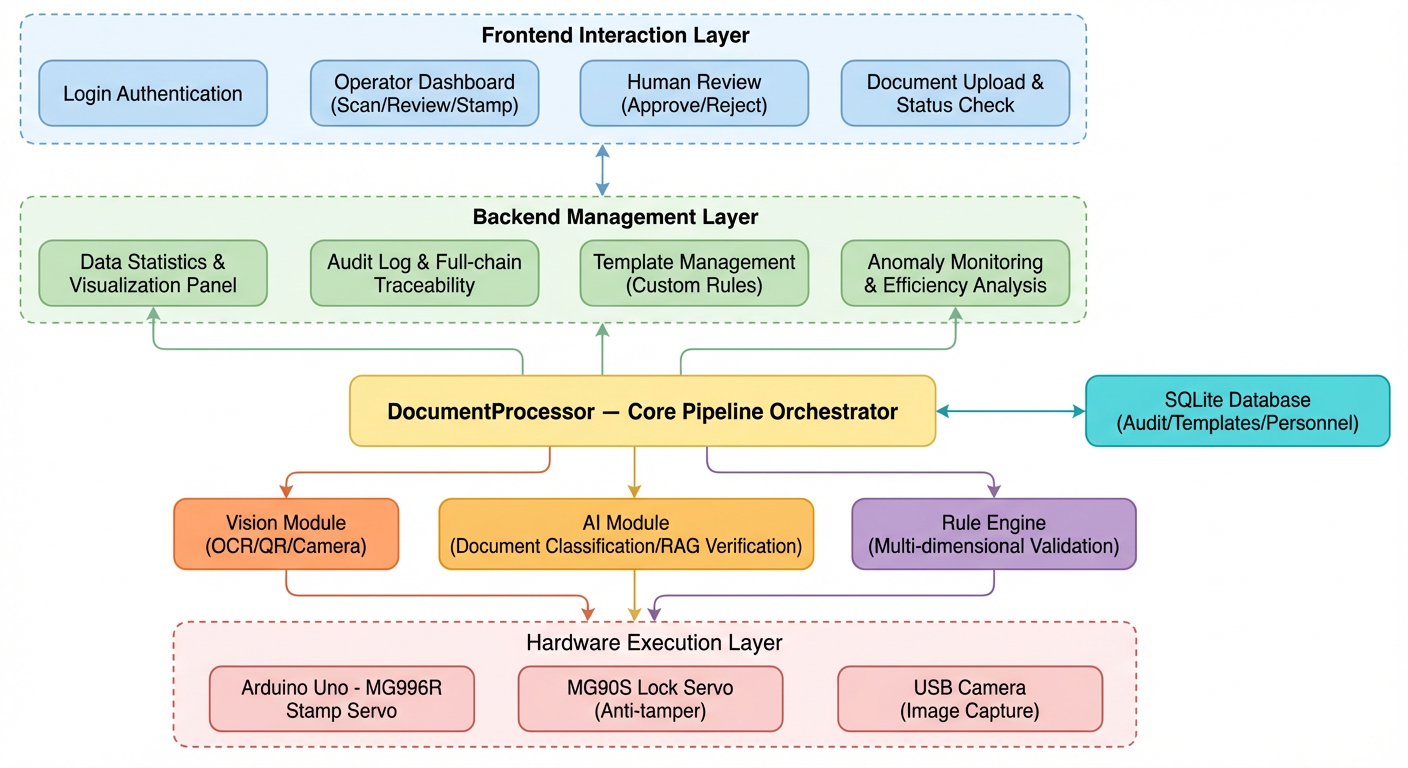
\includegraphics[width=0.85\textwidth]{845afd78c54c4bc0e2f78b941e47ca60.png}
\caption{系统三层架构总览：前端交互层、后台管理层与硬件执行层协同工作，由核心流程编排器统一调度。}
\label{fig:architecture}
\end{figure}

\textbf{第一层——前端交互层}：基于Flask框架构建的Web应用，面向操作员、复审员和管理员三类角色。提供任务提交、文档扫描与审核、人工复审处理、状态查询等交互功能。支持基于角色的访问控制（RBAC），确保不同权限用户只能访问对应功能。

\textbf{第二层——后台管理层}：提供机构运营视角的管理能力，包括：
\begin{itemize}[leftmargin=*]
    \item \textbf{可视化数据统计面板}：实时展示审批通过率、文档类型分布、处理趋势、异常比例等核心运营指标，辅助管理层进行流程优化和资源调配。
    \item \textbf{全链路审计日志}：每份文档的处理过程均记录完整的元数据（操作员、时间戳、OCR结果、验证详情、盖章前后图片），支持按时间、类型、操作员等多维度检索。
    \item \textbf{文档模板管理系统}：管理员可通过可视化界面创建、编辑和删除文档类型模板，定义各文档类型的必填字段、选填字段、非法字段及自定义验证规则，无需修改代码即可扩展系统支持的文档种类。
    \item \textbf{异常监测与效率分析}：自动识别高频拒绝原因、处理瓶颈和异常模式，为流程改进提供数据支撑。
\end{itemize}

\textbf{第三层——硬件执行层}：由Arduino Uno主控板协调USB摄像头、盖章舵机和锁定舵机，完成图像采集和物理盖章操作。通过串口通信（9600波特率）与上层软件系统协同工作。

\subsection{完整处理流程}

系统实现了从文档输入到盖章交付的完整自动化流水线，核心流程包含10个阶段，如\Cref{fig:flowchart}所示。该流程体现了\textbf{输入 $\rightarrow$ 识别 $\rightarrow$ 推理 $\rightarrow$ 决策 $\rightarrow$ 执行 $\rightarrow$ 记录 $\rightarrow$ 分析}的七步闭环设计理念。

\begin{figure}[H]
\centering
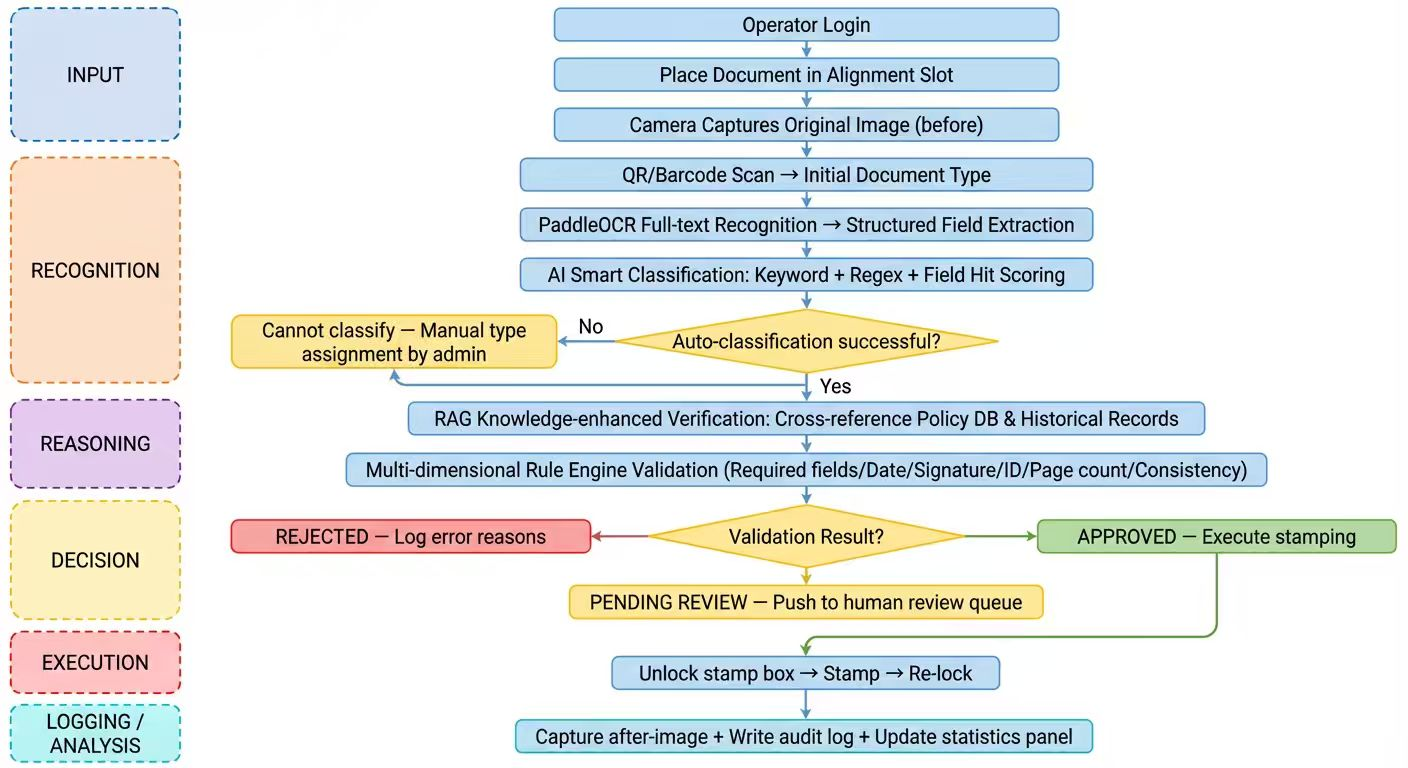
\includegraphics[width=0.85\textwidth]{54b1033c17ddb3bd7cd65716eb862d0e.jpg}
\caption{智能文档处理全流程：七步闭环（输入 $\rightarrow$ 识别 $\rightarrow$ 推理 $\rightarrow$ 决策 $\rightarrow$ 执行 $\rightarrow$ 记录 $\rightarrow$ 分析），三种决策结果——拒绝、人工复审、通过并盖章。}
\label{fig:flowchart}
\end{figure}

\subsection{关键技术组件}

\subsubsection{视觉识别模块}

视觉模块（\texttt{vision/}）负责所有图像采集与文字识别工作，是系统的"感知"入口：

\begin{itemize}[leftmargin=*]
    \item \textbf{摄像头控制}（\texttt{camera.py}）：通过OpenCV管理USB摄像头，自动预热（丢弃前3帧以稳定曝光），使用时间戳命名文件，确保图像采集的一致性和可追溯性。
    \item \textbf{OCR引擎}（\texttt{ocr.py}）：采用PaddleOCR，支持中英文混合识别和角度分类。通过针对中国高校表单优化的正则表达式，将非结构化文本转化为结构化字段（姓名、学号、日期、金额、原因等），为后续验证提供数据基础。
    \item \textbf{二维码扫描}（\texttt{qr\_scanner.py}）：通过pyzbar + OpenCV解码二维码和条形码，实现文档类型的快速初步识别，减少后续AI分类的计算开销。
    \item \textbf{AI文档智能分类}（\texttt{classifier.py}）：当二维码未提供明确文件类型时，系统自动启用AI分类引擎。该引擎采用多特征融合评分策略——\textbf{关键词语义匹配}（权重0.5）、\textbf{正则模式识别}（权重0.3）和\textbf{必填字段命中率}（权重0.5）——对候选文档类型进行综合评分。当最高分与次高分差距小于阈值（0.05）时，系统判定为歧义文档并自动推入人工复审，避免误分类。
\end{itemize}

\subsubsection{RAG知识增强验证模块}

为减少OCR识别幻觉和规则引擎的局限性，系统引入了\textbf{检索增强生成（RAG）}的设计理念，构建了知识辅助验证机制：

\begin{itemize}[leftmargin=*]
    \item \textbf{机构政策知识库}：将各类文档的审批政策、有效期限规定、字段要求等结构化为本地知识库。OCR提取结果与知识库进行交叉检索，验证字段值是否符合当前有效的政策要求。
    \item \textbf{历史审批记录检索}：系统检索相似文档的历史审批结果，辅助判断当前文档是否属于常见异常模式（如频繁出现的字段错误类型），提高异常检测的准确率。
    \item \textbf{幻觉抑制机制}：当OCR提取结果与知识库中的已知约束存在冲突时（如提取的日期格式不符合任何已知日期规范），系统标记为"识别置信度低"并触发人工复审，而非盲目采信OCR输出。
\end{itemize}

\noindent 该设计将纯规则验证升级为\textbf{知识驱动的智能验证}，有效降低了因OCR误识别导致的错误盖章风险。

\subsubsection{多维规则引擎}

验证模块（\texttt{validator/}）实现了基于模板数据库的动态规则引擎，支持管理员通过Web界面自定义验证规则，无需修改代码：

\begin{table}[H]
\centering
\caption{多维验证规则体系及错误分级。}
\label{tab:validation}
\begin{tabular}{@{}llp{4cm}@{}}
\toprule
\textbf{验证维度} & \textbf{实现方式} & \textbf{说明} \\
\midrule
必填字段完整性 & 按文档模板动态检查 & 支持通过模板管理界面配置 \\
日期合法性 & 格式 + 未来日期 + 超期检测 & 超期90天触发软警告 \\
签名/审批栏检测 & OCR文本关键词检索 & 检测签名/审批关键词 \\
ID号交叉验证 & SQLite人员数据库查询 & 学号与姓名匹配验证 \\
文档类型一致性 & QR编码与AI分类结果比对 & 多源验证防止分类错误 \\
多页完整性 & "第X页/共Y页"正则匹配 & 防止缺页提交 \\
非法字段检测 & 模板定义的禁止字段列表 & 检测不应出现的字段 \\
自定义字段规则 & 正则/范围/枚举/长度 & 管理员可配置的灵活规则 \\
\bottomrule
\end{tabular}
\end{table}

\noindent 验证结果分为两级：\textbf{硬错误}（Hard Error）导致立即拒绝；\textbf{软警告}（Soft Warning）将文档推入人工复审队列，由复审员最终裁决，实现人机协同审批。

\subsubsection{硬件执行模块}

硬件模块（\texttt{hardware/stamp.py}）通过串口（9600波特率）与Arduino Uno通信，实现精确的物理盖章控制：

\begin{enumerate}[leftmargin=*]
    \item \textbf{解锁}印章盒（MG90S舵机旋转释放锁扣）。
    \item \textbf{步进式下压}：MG996R舵机以每3\textdegree{}一步、25\,ms间隔缓慢下压，实现力度可控的均匀盖章。
    \item \textbf{停留}900\,ms，确保印迹清晰、墨迹充分转移。
    \item \textbf{缓慢抬起}并\textbf{重新锁定}印章盒，防止非授权使用。
\end{enumerate}

\noindent Arduino固件（\texttt{stamp\_controller.ino}）接受四个串口命令：\texttt{S}（盖章）、\texttt{L}（锁定）、\texttt{U}（解锁）、\texttt{P}（心跳检测），确保软硬件通信的可靠性。

\subsubsection{数据统计与可视化分析}

后台管理平台内置基于Chart.js的数据统计面板，提供以下核心运营指标的可视化分析：

\begin{itemize}[leftmargin=*]
    \item \textbf{汇总指标卡片}：总处理量、通过数量及通过率、拒绝数量及拒绝率、待复审队列长度，一目了然掌握系统运行状态。
    \item \textbf{文档类型分布}：环形图展示各类文档（请假/报销/证明/通用）的提交占比，辅助管理层了解业务构成。
    \item \textbf{审批结果分布}：环形图展示通过/拒绝/待复审的比例，直观反映审批质量。
    \item \textbf{处理趋势分析}：支持7天/30天维度的折线趋势图，展示每日审批量变化，用于识别业务高峰和低谷。
    \item \textbf{最近处理记录}：实时更新的处理流水表格，包含时间、操作员、文档类型和审批结果。
\end{itemize}

\noindent 该分析面板将传统的"黑箱盖章"转化为\textbf{数据驱动的运营管理工具}，使管理层能够基于客观数据优化审批流程、合理分配人力资源，并持续监控系统的运行效率和异常模式。

\subsubsection{异常处理与容错机制}

作为一个涉及软硬件协同的实际部署系统，健壮的异常处理是保证系统可靠运行的关键。系统在\textbf{硬件层、文档识别层和软件系统层}三个维度上设计了完整的容错与降级机制，遵循\textbf{安全优先、优雅降级、人工兜底}的设计原则。

\paragraph{硬件异常处理}

硬件层异常可能导致物理操作失败或安全隐患，因此系统采取了多重保护措施：

\begin{itemize}[leftmargin=*]
    \item \textbf{Arduino连接失败}：系统启动时主动检测串口连接。若连接失败，抛出包含诊断信息的异常（串口号、可能原因排查步骤），指导操作员快速定位问题（USB线松动、端口配置错误、固件未上传等）。
    \item \textbf{盖章过程异常}：盖章序列采用\textbf{异常安全（exception-safe）}设计——\texttt{stamp()}方法在\texttt{try-catch}中执行盖章操作，\textbf{无论成功或失败，均在\texttt{finally}语义下强制执行印章锁定}，防止异常中断导致印章盒处于解锁状态，消除安全隐患。
    \item \textbf{Arduino心跳检测}：系统通过\texttt{P}命令定期检测Arduino在线状态，返回\texttt{PONG}确认通信正常。心跳失败时系统记录告警日志，提示操作员检查硬件连接。
    \item \textbf{摄像头故障}：初始化阶段即检测摄像头是否正常打开（\texttt{isOpened()}），采集阶段捕获读取失败异常并抛出明确错误信息，避免使用空帧图像导致后续OCR产生无效结果。
\end{itemize}

\paragraph{文档内容与格式异常}

文档内容的多样性和不规范是实际部署中遇到的主要挑战，系统通过多级策略进行应对：

\begin{itemize}[leftmargin=*]
    \item \textbf{二维码/条形码缺失}：当文档未粘贴二维码或扫描失败时，系统不直接拒绝，而是\textbf{自动降级到AI智能分类引擎}（\texttt{classifier.py}），通过多特征融合评分判断文档类型，保证流程不中断。
    \item \textbf{AI分类歧义}：当多个文档类型的评分过于接近（差距$<$0.05）时，系统判定为\textbf{歧义文档}，不冒险自动分类，而是推入人工复审队列等待管理员手动指定类型，避免错误分类导致的误判。
    \item \textbf{OCR字段提取不完整}：OCR引擎可能因图像质量、字体差异等原因遗漏字段。系统通过\textbf{必填字段完整性验证}自动检测缺失项，生成具体错误信息（如"缺少必填项：学号"），而非产生不明确的失败。
    \item \textbf{日期格式多样性}：系统支持多种常见中文日期格式的正则匹配（\texttt{YYYY-MM-DD}、\texttt{YYYY年M月D日}、\texttt{YYYY/MM/DD}），并对异常日期（未来日期、年份过早）进行针对性检测，分别归类为硬错误或软警告。
    \item \textbf{学号降级识别}：当标准格式（带"学号"前缀）未命中时，OCR模块\textbf{自动降级到连续数字匹配模式}（8--12位数字），提高识别容错率。
    \item \textbf{多页文档缺页}：通过OCR检测"第X页/共Y页"格式验证多页文档完整性，防止部分页面缺失的文档通过审批。
\end{itemize}

\paragraph{软件系统异常}

\begin{itemize}[leftmargin=*]
    \item \textbf{外部系统集成降级}：DMS（文档管理系统）上传失败时，系统仅记录警告日志，\textbf{不影响本地审批和盖章流程}，确保核心功能不因外部系统不可用而中断。人员信息查询同理，DMS查询失败时自动回退到本地数据库。
    \item \textbf{模板数据库加载失败}：规则引擎尝试从数据库加载文档模板定义，若加载失败则\textbf{自动回退到配置文件中的静态规则}（\texttt{config.py}），保证验证功能始终可用。
    \item \textbf{正则/JSON解析异常}：自定义验证规则中的正则表达式或JSON配置可能存在语法错误，系统对\texttt{re.error}和\texttt{JSONDecodeError}进行捕获，跳过单条出错规则而非导致整个验证流程崩溃。
    \item \textbf{Web API层异常}：Flask路由通过统一的异常捕获返回结构化JSON错误响应（含错误描述和HTTP状态码），前端据此向用户展示友好的错误提示。
    \item \textbf{仿真模式}：系统内置\textbf{SIMULATION\_MODE}配置开关，在无硬件环境下自动跳过所有串口通信，以日志输出替代物理操作，支持开发调试和纯软件演示。
\end{itemize}

\noindent 以上异常处理机制的设计原则可归纳为：\textbf{安全操作必须有兜底}（盖章异常时强制锁定）、\textbf{非核心功能可降级}（DMS、外部查询）、\textbf{不确定结果走人工}（歧义分类、软警告）、\textbf{所有异常均留痕}（写入审计日志），确保系统在面对各类异常时仍能安全、可控地运行。

\subsection{物理结构设计}

设备框架采用\textbf{成本导向的原型验证方案}，使用KT板（A3，5\,mm厚）搭建主体结构。该设计选择基于以下考量：

\begin{itemize}[leftmargin=*]
    \item \textbf{快速迭代}：KT板易于切割和修改，适合在原型阶段快速调整布局和测试不同设计方案。
    \item \textbf{成本控制}：框架材料成本仅15元，验证了系统在极低成本下的可行性，体现项目对\textbf{成本效益}的关注。
    \item \textbf{可移植性}：一旦原型验证完成，主体结构可直接迁移至亚克力、铝合金或钣金等工业化材料，软硬件接口无需修改。
    \item \textbf{避免3D打印依赖}：相较于3D打印方案（单件成本高、打印时间长、不适合批量生产），KT板方案更符合成本控制和面向工业化生产的设计思路。
\end{itemize}

\noindent 设计包括：\textbf{L型对齐挡板}确保纸张定位一致性；\textbf{顶部横梁}安装摄像头俯拍文档；\textbf{侧板安装舵机臂}，印章粘在舵机臂末端；\textbf{防篡改锁定机构}使用副舵机控制物理锁扣。

\begin{figure}[H]
\centering
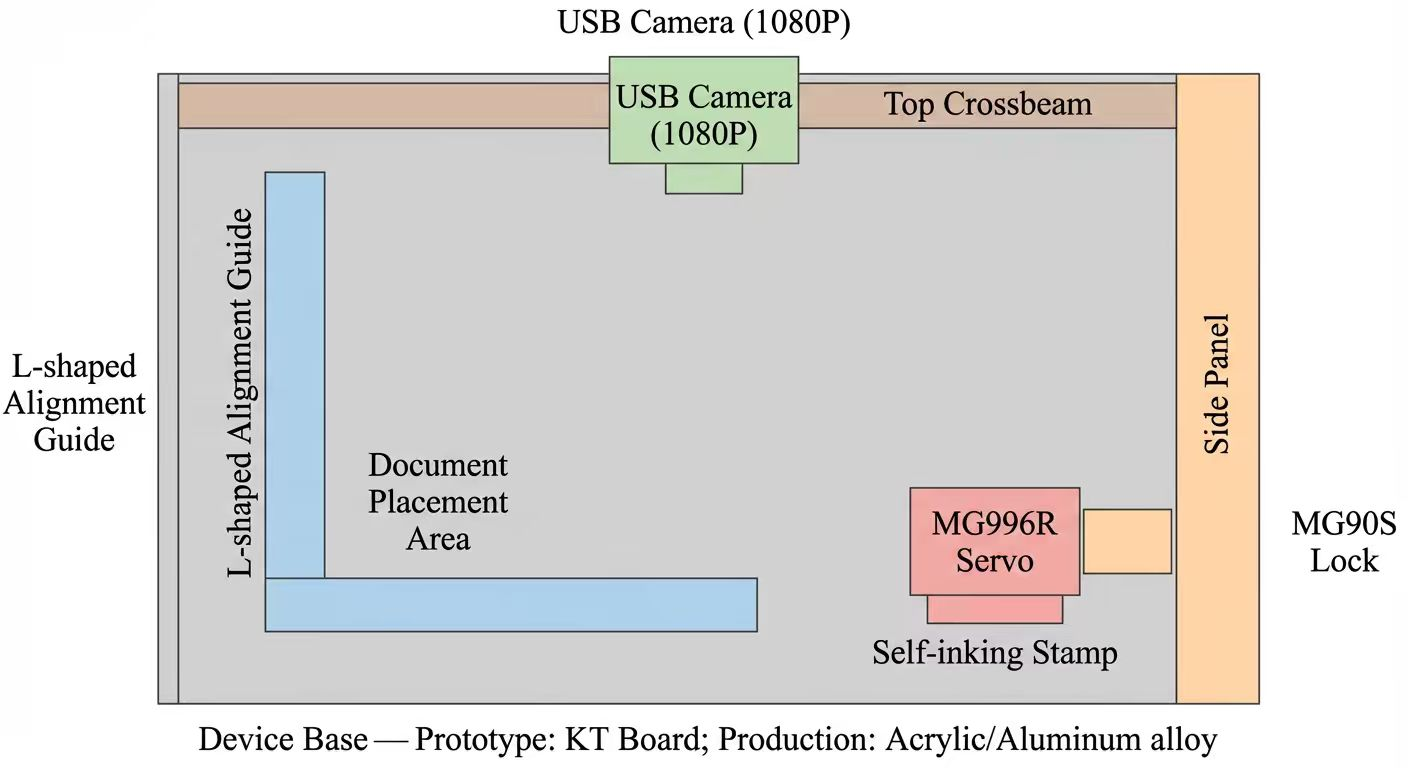
\includegraphics[width=0.7\textwidth]{1909a9044cfacd0bbe122ac6ad0ba1b4.jpg}
\caption{设备框架俯视示意图，展示各组件布局。原型阶段采用KT板，量产阶段可迁移至工业化材料。}
\label{fig:physical}
\end{figure}

%=============================================================================
\section{交付物与目标}
%=============================================================================

\subsection{主要交付物}

\begin{table}[H]
\centering
\caption{项目交付物及验收标准。}
\label{tab:deliverables}
\begin{tabular}{@{}p{4cm}p{4.5cm}c@{}}
\toprule
\textbf{交付物} & \textbf{验收标准} & \textbf{状态} \\
\midrule
AI文档智能分类 & 多特征融合评分，歧义自动标记 & \checkmark \\
OCR结构化字段提取 & 对真实高校表单准确率 $\geq$90\% & \checkmark \\
RAG知识增强验证 & 交叉检索政策库，抑制OCR幻觉 & \checkmark \\
多维规则验证引擎 & 覆盖所有文档类型，支持自定义规则 & \checkmark \\
自动盖章执行 & 舵机步进控制，力度可调，防篡改锁定 & \checkmark \\
人机协同复审队列 & Web端批准/拒绝工作流 & \checkmark \\
可视化统计面板 & 通过率/类型分布/趋势分析 & \checkmark \\
全链路审计日志 & 前后图片 + 完整元数据 + 多维检索 & \checkmark \\
文档模板管理系统 & 可视化创建/编辑模板，零代码扩展 & \checkmark \\
角色权限控制 & operator / reviewer / admin & \checkmark \\
DMS系统集成 & REST API客户端 & \checkmark \\
仿真模式 & 无硬件完整演示 & \checkmark \\
\bottomrule
\end{tabular}
\end{table}

\subsection{开发时间线}

\begin{table}[H]
\centering
\caption{六周开发时间线。}
\label{tab:timeline}
\begin{tabular}{@{}clp{6cm}@{}}
\toprule
\textbf{周次} & \textbf{重点领域} & \textbf{主要活动} \\
\midrule
第1周 & 硬件搭建与基础架构 & 采购元器件，搭建框架，接线Arduino，上传固件，搭建Flask基础框架 \\
第2周 & AI识别与规则引擎 & PaddleOCR集成与调优，AI文档分类器开发，完成多维验证规则 \\
第3周 & Web应用与管理后台 & 构建前端页面（登录/操作台/复审），开发统计面板与模板管理系统 \\
第4周 & 系统集成与RAG验证 & 通过\texttt{main.py}串联所有模块，实现RAG知识检索与幻觉抑制 \\
第5周 & 测试调优与数据分析 & 端到端测试，优化OCR正则和舵机参数，完善统计与异常分析 \\
第6周 & 文档与演示 & 录制演示视频，撰写项目报告，准备答辩 \\
\bottomrule
\end{tabular}
\end{table}

\subsection{团队分工}

\begin{table}[H]
\centering
\caption{团队成员职责与核心交付物。}
\label{tab:team}
\begin{tabular}{@{}llp{3cm}p{3.5cm}@{}}
\toprule
\textbf{成员} & \textbf{角色} & \textbf{核心文件} & \textbf{交付标准} \\
\midrule
甲（硬件） & 框架+Arduino & \texttt{stamp\_controller.ino}, \texttt{hardware/} & 舵机准确盖章，印章对齐，锁定正常 \\
乙（视觉） & OCR+AI分类+摄像头 & \texttt{vision/} & 字段提取 $\geq$90\%，AI分类准确 \\
丙（逻辑） & 规则引擎+RAG验证 & \texttt{validator/}, RAG模块 & 覆盖所有文档类型，幻觉抑制有效 \\
丁（前端） & Web界面+统计面板 & \texttt{web/}, \texttt{templates/} & 全部页面功能完善，可视化面板完整 \\
戊（集成） & 数据库+主流程+模板 & \texttt{main.py}, \texttt{database/} & 端到端流程跑通，模板管理可用 \\
\bottomrule
\end{tabular}
\end{table}

%=============================================================================
\section{所需资源与预算}
%=============================================================================

\subsection{硬件预算}

\begin{table}[H]
\centering
\caption{硬件采购清单及预估费用。}
\label{tab:budget}
\begin{tabular}{@{}cllc@{}}
\toprule
\textbf{\#} & \textbf{器件} & \textbf{规格} & \textbf{费用（元）} \\
\midrule
1 & Arduino Uno R3 & 兼容版 + USB线 & 40 \\
2 & MG996R舵机 & 金属齿轮，10\,kg$\cdot$cm扭矩 & 25 \\
3 & MG90S舵机 & 微型舵机，用于锁定机构 & 15 \\
4 & USB摄像头 & 1080P，广角，免驱 & 60 \\
5 & 光敏印章 & 定制"已审核"刻字，直径4\,cm & 25 \\
6 & KT板 & A3白色，5\,mm，3张 & 15 \\
7 & 热熔胶枪套装 & 含胶棒 & 20 \\
8 & 杜邦线 & 公对母，20\,cm，40根装 & 8 \\
9 & 亚克力盒子 & 小号，印章防篡改存储 & 15 \\
\midrule
 & & \textbf{合计} & \textbf{223元} \\
\bottomrule
\end{tabular}
\end{table}

\subsection{软件技术栈}

所有使用的软件均为开源免费：

\begin{itemize}[leftmargin=*]
    \item \textbf{Python 3.10+} --- 主编程语言
    \item \textbf{PaddleOCR 2.7.3} + \textbf{PaddlePaddle 2.6.1} --- 中文优化OCR引擎
    \item \textbf{Flask 3.0.3} --- Web框架
    \item \textbf{OpenCV 4.9} --- 图像处理
    \item \textbf{Chart.js 4.4} --- 前端数据可视化
    \item \textbf{SQLite 3} --- 嵌入式数据库（无需服务器）
    \item \textbf{Arduino IDE} --- 固件开发
\end{itemize}

\subsection{开发环境}

\begin{itemize}[leftmargin=*]
    \item 操作系统：Windows / macOS / Linux
    \item 内存：4\,GB以上（PaddleOCR模型加载需约1.5\,GB）
    \item 磁盘空间：约500\,MB（含模型和依赖）
    \item 网络：首次运行需下载PaddleOCR模型（约300\,MB）
\end{itemize}

\subsection{预算总结}

项目总预算为1,500元，硬件支出223元，\textbf{剩余1,277元}可用于备用件采购、框架材料升级（如从KT板迁移至亚克力或铝合金）或功能扩展。

%=============================================================================
\section*{贡献分配表}
%=============================================================================

\begin{table}[H]
    \centering
    \caption{个人贡献明细。}
    \label{tab:contribution}
    \begin{tabular}{|c|c|p{6cm}|}
        \hline
        \textbf{学生姓名 / 学号} & \textbf{贡献比例} & \textbf{个人贡献简述} \\
        \hline
        Xinyang Zhang / 2360067 & 20\% & 集成负责人：数据库设计、主流程编排（\texttt{main.py}）、端到端测试 \\
        \hline
        Haoran Zheng / & 20\% & 硬件负责人：物理框架搭建、Arduino固件开发、舵机参数调试与防篡改机构 \\
        \hline
        Yunxuan Wu / & 20\% & 视觉负责人：PaddleOCR集成、AI文档分类器开发、字段提取正则优化 \\
        \hline
        Xiang Lin / & 20\% & 前端负责人：Flask Web应用、可视化统计面板、所有HTML模板与UI设计 \\
        \hline
        Yaokai Yang / & 20\% & 逻辑负责人：多维规则引擎、RAG知识增强验证、复审队列系统与模板管理 \\
        \hline
    \end{tabular}
\end{table}

\end{document}
